\section{Künstliches neuronales Netzwerk\label{ml:ann}}
\rhead{Künstliches neuronales Netzwerk}

\subsubsection{Von linearem Modell zu allgemein nichtlinearem Modell}

Im Abschnitt \ref{ml:regression} haben wird stets ein lineares Modell betrachtet.
Dem Namen ist zu entnehmen, dass es nur lineare Beziehungen abbilden kann. 
Wollen wir Abhängigkeiten höherer Ordnung oder \emph{irgendwelche} nichtlinearen
Abhängigkeiten abbilden, müssen wir dieses Modell erweitern.

Die erste Idee wäre vielleicht das lineare Modell aus
\eqref{ml:regression:modell} viele Male hintereinander zu schalten beziehungsweise zu
verschachteln. Leider \emph{bleibt} aber eine lineare Funktion $k$-mal verschachtelt
linear.

\begin{proof}
    Es wird \eqref{ml:regression:modell} als Funktion
    \begin{equation}
        f_i(\vec x) = \vec y
        = \begin{pmatrix}
            \vec \theta_{1i} \cdot \vec x + b_{1i}\\
            \vdots\\
            \vec \theta_{ni} \cdot \vec x + b_{ni}
        \end{pmatrix}
        = \bm{\thetaup}_i \, \vec x + \vec b_i
       \label{ml:ann:linear-unit}
    \end{equation}
    genommen, wobei der konstante Anteil $\theta_0$ wieder als alleinstehender Term
    geschrieben und $b$ genannt wurde. Zudem hat $f_i(\vec x)$ gleich viele Outputs wie
    Inputs, wodurch $\vec\theta$ zu einer Matrix $\boldsymbol{\thetaup}$ und der Skalar
    $b$ zu einem Vektor $\vec b$ werden.
    
    Streng genommen ist diese Funktion nicht mehr linear im allgemeinen mathematischen
    Sinn, denn das Superpositionsprinzip gilt durch den konstanten Anteil $\vec b_i$ nicht
    mehr (im Sinne der linearen Algebra sind es affine Abbildungen und nicht lineare, die
    lineare Abbildung ist eine spezielle affine Abbildung). Der Begriff Linearität wird
    hier vielmehr im Bezug auf lineare Funktionen verwendet.

    Können wir zeigen, dass die lineare Funktion $f_i$ einmal verschachtelt wieder eine
    lineare Funktion ergibt, ist das auch für beliebig viele Verschachtelungen der Fall.
    
    Es wird $f_i$ einmal verschachtelt und ausmultipliziert:
    \begin{equation}
    \begin{aligned}
        \vec y_2 &= f_2(f_1(\vec x)) = (f_2 \circ f_1)(\vec x)
            = {\bm \thetaup}_2 ({\bm \thetaup}_1 \vec x + \vec b_1) + \vec b_2\\
        &= \underbrace{{\bm \thetaup}_2 {\bm \thetaup}_1}_{\tilde {\boldsymbol\thetaup}_1} \vec x
            + \underbrace{{\bm \thetaup}_2 \vec b_1 + \vec b_2}_{\tilde{\vec b}_1}
            = \tilde {\boldsymbol\thetaup}_1 \vec x + \tilde{\vec b}_1
    \end{aligned}
    \label{ml:ann:lin-comp-proof}
    \end{equation}
    Wie \eqref{ml:ann:lin-comp-proof} zeigt ist also möglich $f_2 \circ f_1$ wieder als lineare Funktion zu schreiben.
\end{proof}

\subsection{Aktivierungsfunktion}

Um Nichtlinearitäten einzubauen wird eine sogenannte \emph{activation function} auf
\eqref{ml:ann:linear-unit} angewendet. Die Koeffizienten-Matrix ${\bm \thetaup}$ soll
immer noch mit \hyperref[ml:regression:gd]{Gradient-Descent} gelernt werden, also muss
die gewählte Aktivierungsfunktion ableitbar bezüglich aller Inputs sein.

Es gibt viele mögliche Aktivierungsfunktionen. Eine der ersten die gebraucht wurde ist die \emph{Sigmoid}-Funktion
\begin{equation}
    \sigma(y) = \frac{1}{1+e^{-y}} \quad
    \text{mit der einfachen Ableitung}\quad
    \sigma'(y) = \sigma(y)(1- \sigma(y)).
    \label{ml:ann:activation:sigmoid}
\end{equation}

$\sigma(y)$ wird nun auf $f_i$ \emph{elementweise} angewendet, also
\begin{equation}
    g_i(\vec x) = \sigma(f_i(\vec x)) = \sigma({\bm \thetaup}_i \vec x + \vec b_i)
    = \begin{pmatrix}
        \sigma \left( \vec \theta_{1i} \cdot \vec x + b_{1i} \right)\\
        \vdots\\
        \sigma \left( \vec \theta_{ni} \cdot \vec x + b_{ni} \right)
    \end{pmatrix}.
    \label{ml:ann:one-layer}
\end{equation}

Es existieren viele weitere praktische Aktivierungsfunktionen mit guten und schlechten Eigenschaften für
eine Problemstellung, auf diese soll hier nicht weiter eingegangen werden.

\subsection{Multilayer ANN}

Für das vollständige nichtlineare Modell wird $g_i$ $k$-mal verschachtelt:
\begin{equation}
    M({\bm \thetaup}_1, \cdots, {\bm \thetaup}_n, \vec b_1, \cdots, \vec b_n) = \vec y
        = (g_1 \circ g_2 \circ \cdots \circ g_n)(\vec x) = g_n(g_{n-1}(\cdots g_1(\vec x))).
    \label{ml:ann:multilayer}
\end{equation}
So ein Modell $M$ wird \emph{fully connected feedforward artificial neural network}\footnote{
    Bei dieser Netzwerk-Struktur sind alle Neuronen einer Schicht mit \emph{allen} der
    nächsten Schicht vollverbunden. Die feedforward Struktur impliziert fast immer auch
    die volle Verbundenheit und wird deshalb im weiteren Text weggelassen.
} (FFANN) genannt.

Was genau bei der numerischen Berechnung passiert ist viel einfacher
in Form eines gerichteten Graphen in Abb. \ref{fig:ml:ann:simple} zu erkennen.

\begin{figure}
    \centering
    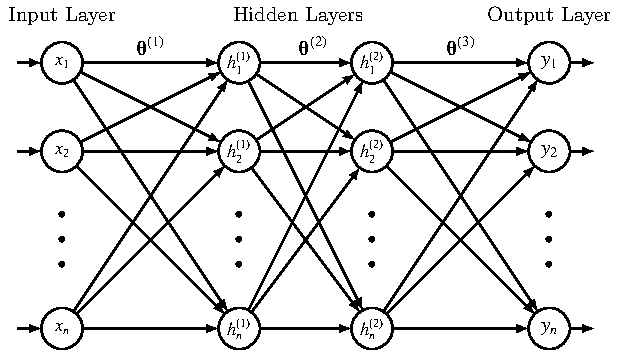
\includegraphics[scale=0.8]{papers/ml/images/ann_simple.pdf}
    \caption{3-schichtiges FFANN in Form eines gerichteten Graphen.}
    \label{fig:ml:ann:simple}
\end{figure}

Das Modell wird mit geschichteten Neuronen dargestellt, dabei sind bei dieser
Netzwerk-Struktur alle Neuronen einer vorherigen Schicht mit allen der nächsten verbunden.
Die Kanten zwischen den Neuronen stellen die Gewichte in der $\bm \thetaup$-Matrix
dar. Die Schichten zwischen der Eingangs- und Ausgangsschicht werden \emph{hidden layer}
genannt, da all diese Layer nicht von aussen gesehen oder angesprochen werden können.

Auf der linken Seite des Diagramms sind die Eingänge. Sie werden mit dem entsprechenden
Gewicht $\theta^{(i)}_k$ der Kante gewichtet. Anschliessend werden die gewichteten Werte
aller eingehenden Kanten plus einer Konstante $b^{(i)}_k$ summiert und darauf die
Aktivierungsfunktion der Neurone angewendet. Das Resultat ist der Eingangswert
für die nächste Schicht.

Diese Berechnung propagiert so von links nach rechts durch das Netzwerk bis am Ende die
Werte bei der Ausgangsschicht anliegen.

Die Struktur des Netzwerks, also die Anzahl Eingänge, Hidden-Layer, Neuronen
pro Layer und Ausgänge, aber auch die spezifischen Aktivierungsfunktionen können
grundsätzlich frei gewählt werden. Sie werden \emph{hyperparameter} genannt.

\subsection{Backpropagation \label{ml:ann:backpropagation}}

Wir wollen den \hyperref[ml:regression:gd]{Gradient-Descent-Algorithmus} auch auf
unser nichtlineares Modell $M$ aus \eqref{ml:ann:multilayer} anwenden. Damit ist es aber nicht
mehr so einfach wie mit dem linearen Modell von vorher. 
$M$ besteht aus mehreren Layern, jeder mit einer Koeffizientenmatrix $\bm \thetaup$ und einem
Bias-Vektor $\vec b$. All diese Werte sollen iterativ mit Gradient-Descent gelernt werden,
sodass alle Outputs des gesamten Netzwerks möglichst nahe an den geforderten sind.

Um diese Problemstellung zu untersuchen beschränken wir uns zuerst auf den Fall eines
Netzwerks mit \emph{einem} Eingang, $n$ Hidden-Layer mit \emph{einem} Neuron und
\emph{einem} Ausgang. Mit dieser Forderung wird die Matrizengleichung
\eqref{ml:ann:multilayer} zu einer skalaren Gleichung
\begin{equation}
    M(x, \theta_1, \cdots, \theta_n, b_1, \cdots, b_n)
    = \sigma(\theta_n \cdot \sigma( \theta_{n-1}
        \cdot \sigma ( \cdots \sigma( \theta_1 x + b_1 ) ) + b_{n-1} ) + b_n).
    \label{ml:ann:multilayer-1D}
\end{equation}
Abbildung \ref{fig:ml:ann:simple-1D} zeigt \eqref{ml:ann:multilayer-1D} wieder als
gerichteten Graphen.

\begin{figure}
    \centering
    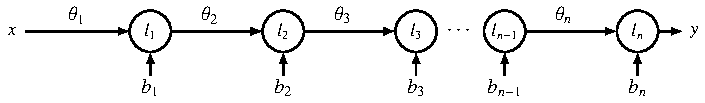
\includegraphics[scale=0.8]{papers/ml/images/ann_simple_1D.pdf}
    \caption{Eindimensionales FFANN.}
    \label{fig:ml:ann:simple-1D}
\end{figure}

$\theta_i$ sind die Gewichte (englisch \emph{weights}) der Verbindungen beziehungsweise
Kanten zwischen den Neuronen, $b_i$ sind die konstanten Anteile (englisch \emph{biases})
und $\sigma$ ist die Aktivierungsfunktion der Neuronen. Jedes $l_i$ soll den Output eines
Layers darstellen.

Zur weiteren Verdeutlichung wird \eqref{ml:ann:multilayer-1D} als Gleichungssystem
geschrieben:
\begin{equation}
    \begin{aligned}
        l_1 &= \sigma(\theta_1 x + b_1) = \sigma(\xi_1)\\
        l_2 &= \sigma(\theta_2 l_1 + b_2) = \sigma(\xi_2)\\
        &\hspace{1.5cm}\vdots\\
        y=l_n &= \sigma(\theta_n l_{n-1} + b_n) = \sigma(\xi_n)\\
    \end{aligned}
    \qquad\text{mit}\qquad
    \xi_i = \theta_i l_{i-1} + b_i
    .
\end{equation}

Wie schon bei Gradient-Descent im linearen Fall soll wieder die Cost-Function $J(\theta,b)
= (y - M(x, \theta, b))^2$ minimiert werden. Wir verwenden hier die selbe Cost-Function
wie in Abschnitt \ref{ml:regression}, in der Praxis kann aber irgendeine günstige
\emph{ableitbare} Funktion verwendet werden.

Es wird wieder der Gradient von $J$ gebildet, wobei die entgegengesetzte Richtung immer
noch zu einem lokalen Minimum führt. Der Gradient beinhaltet die partiellen Ableitungen
bezüglich aller Parameter

\begin{equation}
    \frac{\partial J}{\partial \theta_i} = 2(M(x) - y) \cdot \frac{\partial M}{\partial \theta_i}
    \qquad\text{und}\qquad
    \frac{\partial J}{\partial b_i} = 2(M(x) - y) \cdot \frac{\partial M}{\partial b_i}.
\end{equation}

Mit der Kettenregel
\begin{equation}
    \frac{d}{dt}f(g(t)) = \frac{df(g(t))}{d g(t)} \cdot \frac{d g(t)}{dt} = \frac{df(\tau)}{d \tau} \cdot \frac{d g(t)}{dt}
\end{equation}
lassen sich die partiellen Ableitungen von $M$ einfach berechnen.
\[
\begin{aligned}
    \frac{\partial M}{\partial \theta_n} &= \frac{\partial l_n}{\partial \theta_n} =
    \sigma'(\theta_n l_{n-1} + b_n) l_{n-1} = \sigma'(\xi_n)l_{n-1} \\
    \frac{\partial M}{\partial \theta_{n-1}} &= \frac{\partial l_{n}}{\partial \theta_{n-1}}
    = \frac{\partial l_n}{\partial l_{n-1}} \cdot \frac{\partial
    l_{n-1}}{\partial \theta_{n-1}} = 
    \sigma'(\xi_n) \theta_n \cdot \sigma'(\xi_{n-1}) l_{n-2}
    \\
    \frac{\partial M}{\partial \theta_{n-2}} &= \frac{\partial l_{n}}{\partial \theta_{n-2}}
    = \frac{\partial l_n}{\partial l_{n-1}} \cdot \frac{\partial
    l_{n-1}}{\partial l_{n-2}}\cdot \frac{\partial l_{n-2}}{\partial \theta_{n-2}} =
    \; \sigma'(\xi_n)\theta_n \cdot \sigma'(\xi_{n-1})\theta_{n-1}\cdot \sigma'(\xi_{n-2})l_{n-3}
    \\
    \vdots\quad&\\
    \frac{\partial M}{\partial b_n} &= \frac{\partial l_n}{\partial b_n} =
    \sigma'(\xi_n) \\
    \frac{\partial M}{\partial b_{n-1}} &= \frac{\partial l_{n}}{\partial b_{n-1}}
    = \frac{\partial l_n}{\partial l_{n-1}} \cdot \frac{\partial
    l_{n-1}}{\partial b_{n-1}} = 
    \sigma'(\xi_n) \theta_n \cdot \sigma'(\xi_{n-1}) \\
    \vdots\quad&
\end{aligned}
\]

Wichtig zu erkennen ist, dass alle Werte $l_i$ sowie auch $\xi_i=\theta_i l_{i-1}+b_i$ nur
einmal berechnet werden müssen. Das Netzwerk muss sowieso für den finalen Wert $y$ einmal
ausgewertet werden, dieser Schritt wird \emph{forward propagation} (deutsch Vorwärtspropagierung)
genannt. Gleichzeitig können alle Zwischenresultate gespeichert werden, um sie für den
Korrekturschritt direkt einzusetzen.

Die Parameter werden analog zu \eqref{ml:regression:gd:update} bei jeder Iteration mit
\begin{equation}
    \theta_i \leftarrow \theta_i - \alpha \frac{\partial J}{\partial \theta_i}
    \qquad\text{und}\qquad
    b_i \leftarrow b_i - \alpha \frac{\partial J}{\partial b_i}
\end{equation}
angepasst.

Bei den partiellen Ableitungen sieht man, das jede Schicht $i$ immer von allen
nächsten Schichten $i+1, i+2, \cdots$ mit identischer Form abhängt. Gibt es also eine Formel
die nur den Zusammenhang zwischen zwei Neuronen beschreibt? Klar, die gibt's.

Wir führen dazu die neue Grösse 
\begin{equation}
    \delta_i = \frac{\partial J}{\partial \xi_i}
\end{equation}
ein, sie wird auch \emph{local gradient} (deutsch lokaler Gradient) genannt. Damit können
die partiellen Ableitungen und Aktualisierungsgleichungen schon einmal vereinfacht geschrieben werden:
\begin{equation}
    \frac{\partial J}{\partial \theta_i} = \delta_i \cdot l_{i-1}
    \;\Rightarrow\; \Delta \theta_i = - \alpha \delta_i l_{i-1}
    \qquad\text{und}\qquad
    \frac{\partial J}{\partial b_i} = \delta_i
    \; \Rightarrow\; \Delta b_i = - \alpha \delta_i.
\end{equation}

Der lokale Gradient kann schliesslich mit
\begin{equation}
    \delta_{i-1} = \frac{\partial J}{\partial \xi_i} \cdot \frac{\partial \xi_i}{\partial \xi_{i-1}}
    = \delta_i \cdot \frac{\partial \xi_i}{\partial \xi_{i-1}}
    = \delta_i \cdot \sigma'(\xi_{i-1}) \theta_i
    \label{ml:ann:bp:rekursiv}.
\end{equation}
rekursiv berechnet werden. In \eqref{ml:ann:bp:rekursiv} ist noch besser zu erkennen, dass das Übertragungsverhalten
des Fehlers $\delta_{i-1}/\delta_i$
zwischen zwei Neuronen von zwei benachbarten Schichten $i$ und $i+1$ nur von der Kante
$(i)\rightarrow(i+1)$ dazwischen (also dem
Gewicht), der Ableitung der Aktivierungsfunktion des Neuron in Schicht $i$ und dem lokalen
Gradienten der Schicht $i+1$ abhängt.
$\delta_n$ der letzten Schicht berechnet sich noch mit der normalen Formel
\begin{equation}
    \delta_n = \frac{\partial J}{\partial \xi_n}
    = \frac{\partial J}{\partial M} \cdot \frac{\partial M}{\partial \xi_n}
    = 2(\underbrace{M(x)}_{l_n} - y) \cdot \sigma'(\xi_n).
\end{equation}

Die rekursive Berechnung des Fehlergradienten und somit der Anpassungsinformation für alle
Gewichte und Konstanten ist, wie wir gesehen haben, extrem simpel und performant.
Dieser Anpassungsprozess als Rückpropagierung des Fehlers wird \emph{backpropagation} genannt.

\subsubsection{Erweiterung auf allgemeine feedforward Netzwerke}

Wir haben in der Herleitung vom Backpropagation-Algorithmus ein stark vereinfachtes
Netzwerk betrachtet. Mit den gleichen Überlegungen ist es aber auch möglich
Backpropagation für ein Netzwerk mit mehreren Ein- und Ausgängen, mehreren Neuronen pro
Hidden-Layer und verschiedenen Aktivierungsfunktionen zu machen.

Durch Summierung der Kosten aller Ausgänge kann erst einmal die Cost-Function sehr einfach
auf mehrere Outputs erweitert werden:
\[
    \tilde J(\theta, b) = \sum_{k\in \text{Outputs}} J(M_k(x), y).
\]
Danach können die Backpropagation-Gleichungen analog aufgestellt werden:
\begin{equation}
\begin{aligned}
    \delta_{\text{node}_i}^{(\text{last layer})} &=
        \frac{\partial \tilde J}{\partial \xi_{\text{node}_i}^{(\text{last layer})}} \\
    \delta_{\text{node}_k}^{(\text{previous layer})} &=
        \sigma'_{\text{node}_k} \left( \xi_{\text{node}_k}^{(\text{previous layer})} \right) 
        \sum_{j\in \substack{\text{nodes of}\\\text{current layer}}}
        \theta_{k\rightarrow j} \cdot \delta_j\\
    \theta_{\text{node}_k\rightarrow\text{node}_j} &\leftarrow
        \theta_{\text{node}_k\rightarrow\text{node}_j} -
        \alpha \cdot \delta_{\text{node}_j} \cdot \sigma_{\text{node}_k}(\xi_{\text{node}_k}) \\
    b_{\text{node}_j} &\leftarrow b_{\text{node}_j} - \alpha \cdot \delta_{\text{node}_j}
\end{aligned}.
\label{ml:ann:bp:update}
\end{equation}

\bigskip
Unser Ziel eines universellen Approximators ist somit erreicht. In der Praxis sind die
Algorithmen für Gradient-Descent, Backpropagation und verbesserte Ableger davon in
Bibliotheken implementiert. Einige bekannte Bibliotheken für die Programmiersprache Python
sind \texttt{Keras}, \texttt{TensorFlow} und \texttt{PyTorch}.